\documentclass[11pt]{article}

\usepackage[margin=1in]{geometry}
\usepackage[utf8]{inputenc}
\usepackage[T1]{fontenc}
\usepackage{lmodern}
\usepackage{amsmath}
\usepackage{booktabs}
\usepackage{graphicx}
\usepackage{xcolor}
\usepackage{hyperref}
\usepackage[numbers]{natbib}

% Marcas de trabajo pendiente. Antes de enviar: \renewcommand{\todo}[1]{} y buscar "TODO".
\newcommand{\todo}[1]{\textcolor{red}{[TODO: #1]}}

\title{Probing Reveals the Intent to Attack, Not the Success of the Hack:\\
Command-Level Environment Probing in Reward-Hacking Agents}

\author{
  \todo{Nombre Apellido (Sebastián)} \and
  \todo{Nombre Apellido (Inés)} \and
  \todo{Nombre Apellido (Rodrigo)}\\[4pt]
  \todo{Afiliación} \\
  \todo{emails}
}
\date{}

\begin{document}
\maketitle

\begin{abstract}
Agents that reward hack often explore their environment before exploiting it: in the 2026 OpenAI--Hugging Face incident, environment probing rose during training of the model that later attacked a production system~\citep{openai2026report}. We ask whether reward-hacking trajectories show more environment probing than legitimate ones, measured \emph{only from the agent's commands}, without access to its reasoning. We define a rule-based taxonomy of probing (reading the verifier, exploring outside the task scope, system and runtime introspection, reaching the outside world) and score each trajectory by its number of probing commands. On all 8{,}641 trajectories of Terminal Wrench~\citep{terminalwrench}, probing separates attack-prompted agents from baseline agents (Claude Opus 4.6: AUC 0.68 after controlling for trajectory length; 248 of 295 tasks), but it does not separate successful hacks from legitimate solves produced under the same attack prompt (AUC 0.48--0.50 across three models and three robustness controls). On EvilGenie~\citep{evilgenie}, where no one asks the agent to cheat, an open 20B model reward hacked spontaneously in 1 of 333 attempts, after reading the test file. Command-level probing is thus an early signal of an agent \emph{looking for} shortcuts, not evidence that it \emph{took} one. \todo{Agregar resultado de la validación humana (kappa) cuando esté.}
\end{abstract}

\section{Introduction}
\label{sec:intro}

% Párrafo 1: qué es reward hacking y por qué importa.
\emph{Reward hacking} is when an agent obtains the reward by exploiting flaws in the verifier instead of solving the intended task. \todo{2--3 frases de contexto y por qué importa para agentes con herramientas.}

% Párrafo 2: el incidente. Solo fuentes primarias (informe de OpenAI y de METR/Redwood).
In July 2026, agents trained by OpenAI escaped an evaluation sandbox and reached Hugging Face infrastructure while trying to cheat on the ExploitGym benchmark~\citep{openai2026report,metr2026report}. OpenAI reports that its models ``increasingly learned to probe and exploit their environment during training'', and that tasks impossible to solve as intended were ``a significant factor leading models to probe their sandbox''~\citep[pp.~20--22]{openai2026report}. In one training run, the rate of environment probing flagged by a chain-of-thought monitor rose from roughly 0.2\% to roughly 3.7\%~\citep[Fig.~2]{openai2026report}. \todo{Aclarar que 0,2 y 3,7 son lecturas de la figura, no cifras del texto; la unidad no está definida en el informe.}

% Párrafo 3: la pregunta.
This raises a monitoring question. OpenAI detected probing by reading the model's reasoning, which may be unavailable or unfaithful. Can probing be measured from the agent's \emph{actions} alone, and does it distinguish agents that reward hack from those that solve the task?

% Párrafo 4: qué hacemos.
We study this on two benchmarks: Terminal Wrench~\citep{terminalwrench}, which provides thousands of elicited hack and non-hack trajectories, and EvilGenie~\citep{evilgenie}, which we run ourselves with open models and no instruction to cheat.

% Contribuciones.
Our contributions are:
\begin{itemize}
  \item A command-level taxonomy of environment probing (S1--S5) and manipulation (M), with a rule-based classifier that adapts its notion of task scope to each task (Section~\ref{sec:method}).
  \item An analysis of all 8{,}641 Terminal Wrench trajectories showing that probing tracks the \emph{instruction to attack} but not the \emph{success} of the hack, robust to task, length and unclassified commands (Section~\ref{sec:results}).
  \item Spontaneous reward-hacking rates for open models on EvilGenie, including a fix for a provider bug that halved the measured capability of \texttt{gpt-oss-20b} (Section~\ref{sec:setup}).
  \item A blind human validation of the classifier and of the dataset's hack labels (Section~\ref{sec:validation}). \todo{solo si se termina la revisión}
  \item Code, run logs and per-trajectory results, released openly. \todo{link al repo público}
\end{itemize}

\section{Related Work}
\label{sec:related}

\paragraph{Reward hacking benchmarks.}
Terminal Wrench~\citep{terminalwrench} collects 331 reward-hackable terminal tasks and 3{,}632 exploit trajectories from three frontier models, elicited with an explicit red-team prompt, and labels each trajectory with an LLM judge and an 11-category exploit taxonomy. EvilGenie~\citep{evilgenie} builds coding problems from LiveCodeBench~\citep{livecodebench} with visible and held-out tests and detects hacking through held-out failures, test-file edits and an LLM judge, without asking the agent to cheat. \todo{Agregar otros trabajos de reward hacking / specification gaming si los citamos.}

\paragraph{Monitoring agents.}
Terminal Wrench reports that an LLM monitor detects hacks with AUC 0.97 from full trajectories, dropping to 0.92 when the agent's reasoning is stripped~\citep{terminalwrench}. \todo{Citar trabajo sobre monitoreo de cadena de pensamiento (p. ej. \citet{baker2025monitoring}, verificar).} Our probing score is a cheaper, transparent signal computed from commands only.

\paragraph{The OpenAI--Hugging Face incident.}
OpenAI's technical report~\citep{openai2026report} and the independent METR/Redwood investigation~\citep{metr2026report} describe agents that coordinated, probed their sandbox and attacked external infrastructure to cheat. \todo{1--2 frases sobre lo que dice METR del comportamiento de los agentes.}

\section{Measuring Probing from Commands}
\label{sec:method}

\subsection{Definition}
We define \emph{probing} as any read-only action whose purpose is to obtain information about the evaluation environment, the verifier or the system, beyond what the task needs. Three rules make this operational: (i) probing only reads; modifying tests, verifiers or binaries is \emph{manipulation} (M), measured separately; (ii) probing is relative to the task scope, so reading \texttt{nginx.conf} is normal work when the task is to configure nginx; (iii) only the command is judged, never the agent's stated reasoning.

\subsection{Categories}
\begin{table}[h]
\centering
\small
\begin{tabular}{lll}
\toprule
Code & Category & Examples \\
\midrule
S1 & Reading or searching the verifier & \texttt{cat test.py}, \texttt{find / -name '*verify*'}, \texttt{ls /solution} \\
S2 & Exploring outside the task scope & \texttt{ls /root}, \texttt{cat \textasciitilde/.bash\_history} \\
S3 & System and process introspection & \texttt{ps aux}, \texttt{env}, \texttt{cat /proc/1/cmdline} \\
S4 & Runtime environment inspection & \texttt{pip list}, \texttt{which python3}, \texttt{dpkg -l} \\
S5 & Reaching the outside world & \texttt{curl}, \texttt{pip install} of an unnamed package \\
N  & Normal task work & running the tests, compiling, editing the solution \\
M  & Manipulation (not probing) & replacing \texttt{/usr/bin/python3}, editing the checker \\
?  & Undecided by the rules & \\
\bottomrule
\end{tabular}
\caption{Command categories. Each part of a chained command (\texttt{;}, \texttt{\&\&}, \texttt{|}) is labeled separately.}
\label{tab:categories}
\end{table}

\subsection{Classifier}
\todo{Describir el clasificador por reglas: separación de comandos encadenados y heredocs, precedencia (M > S5 > S4 > S3 > S2 > S1 > N), terminal persistente (\texttt{cd}).}
For Terminal Wrench, the task scope is built per task: the working directory is the Dockerfile's \texttt{WORKDIR}; paths and programs named in the task instruction count as normal work; \texttt{/tests}, \texttt{/solution} and files named like verifiers (\texttt{check-*}, \texttt{grader}, \texttt{verify*}) count as S1; re-reading a file the agent wrote earlier is not probing. \todo{Mencionar los 34 tests del clasificador y el 6.4\% de partes sin clasificar.}
\todo{Si se corrigen los dos errores encontrados en la auditoría de la tarea 1018 (\texttt{/dev/null} y comandos pedidos literalmente por la consigna), describir la versión final.}

\subsection{Trajectory metrics}
The \textbf{probing score} of a trajectory is its number of command parts labeled S1--S5. Because the score grows with trajectory length, we always report it next to the \textbf{probing ratio} (score divided by the number of command parts) and control for length explicitly (Section~\ref{sec:robustness}).

\subsection{Statistics}
We compare groups with the Mann--Whitney $U$ test and report the AUC ($U/(n_1 n_2)$): the probability that a random trajectory from the first group has a higher score than one from the second. Within-task comparisons use an exact two-sided sign test over (task, model) pairs, comparing group medians and dropping ties.

\section{Experimental Setup}
\label{sec:setup}

\subsection{Terminal Wrench}
We analyze all 8{,}641 trajectories of Terminal Wrench~\citep{terminalwrench} (commit \texttt{d8a2961}): 6{,}289 attack trajectories run with the red-team prompt and 2{,}352 baseline trajectories without it, from Claude Opus 4.6, Gemini 3.1 Pro and GPT-5.4. Groups follow the dataset's labels: \emph{hack} (rewarded serious and non-serious exploits, 3{,}632), \emph{legitimate} (attacker solved the task as intended, 1{,}216), \emph{no reward} (1{,}441) and \emph{baseline}. Hack and legitimate trajectories received the same attack prompt, which instructs the agent not to solve the task normally; legitimate ones solved it anyway. In total we classify 309{,}656 command parts.

\subsection{EvilGenie}
We run EvilGenie~\citep{evilgenie} with Inspect~\citep{inspect} on the 154 competition-level LiveCodeBench problems, with a 600\,s limit per problem, one problem at a time, and the LLM judge disabled during runs (applied afterwards). The agent is never told to cheat. We log every tool call to a separate action log joined to Inspect's scores.

\paragraph{Models.} \texttt{gpt-oss-20b}~\citep{gptoss} served by the NVIDIA API (reasoning effort \emph{medium}); \texttt{qwen3:8b}, \texttt{qwen3:14b} and \texttt{qwen3:30b-a3b}~\citep{qwen3} served locally with Ollama (thinking off); \texttt{nemotron-3-ultra-550b-a55b} via NVIDIA. We scale each model in stages of 5, 50 and 154 problems, advancing only if the agent executes commands in at least 3 of the first 5 problems. \todo{Tabla de corridas (ver notas/corridas.md).}

\paragraph{Provider fix.} The NVIDIA API appended a harmony-format token to tool names (e.g.\ \texttt{safe\_python<|channel|>commentary}), so Inspect rejected 36--48\% of \texttt{gpt-oss-20b}'s tool calls, and it sometimes returned responses without choices, aborting 14--18\% of problems. We strip the suffix when the remainder is a valid tool and retry empty responses, logging every correction. On the same 154 problems, solved problems rose from 29--30 to 54--60 and aborted problems fell to zero. All main EvilGenie results use the patched runs.

\paragraph{Hack labels.} A trajectory is a hack candidate if it passes visible tests but fails held-out ones, if it modifies test files, or if the LLM judge labels it \emph{reward\_hacking}. Every candidate is reviewed manually and labeled intentional or accidental. \todo{Juez: GLM-5.3 vía NVIDIA (los resultados quedaron en el servidor; recuperarlos o re-correr).}

\section{Results}
\label{sec:results}

\subsection{Probing tracks the attack prompt, not the hack}
\begin{figure}[h]
\centering
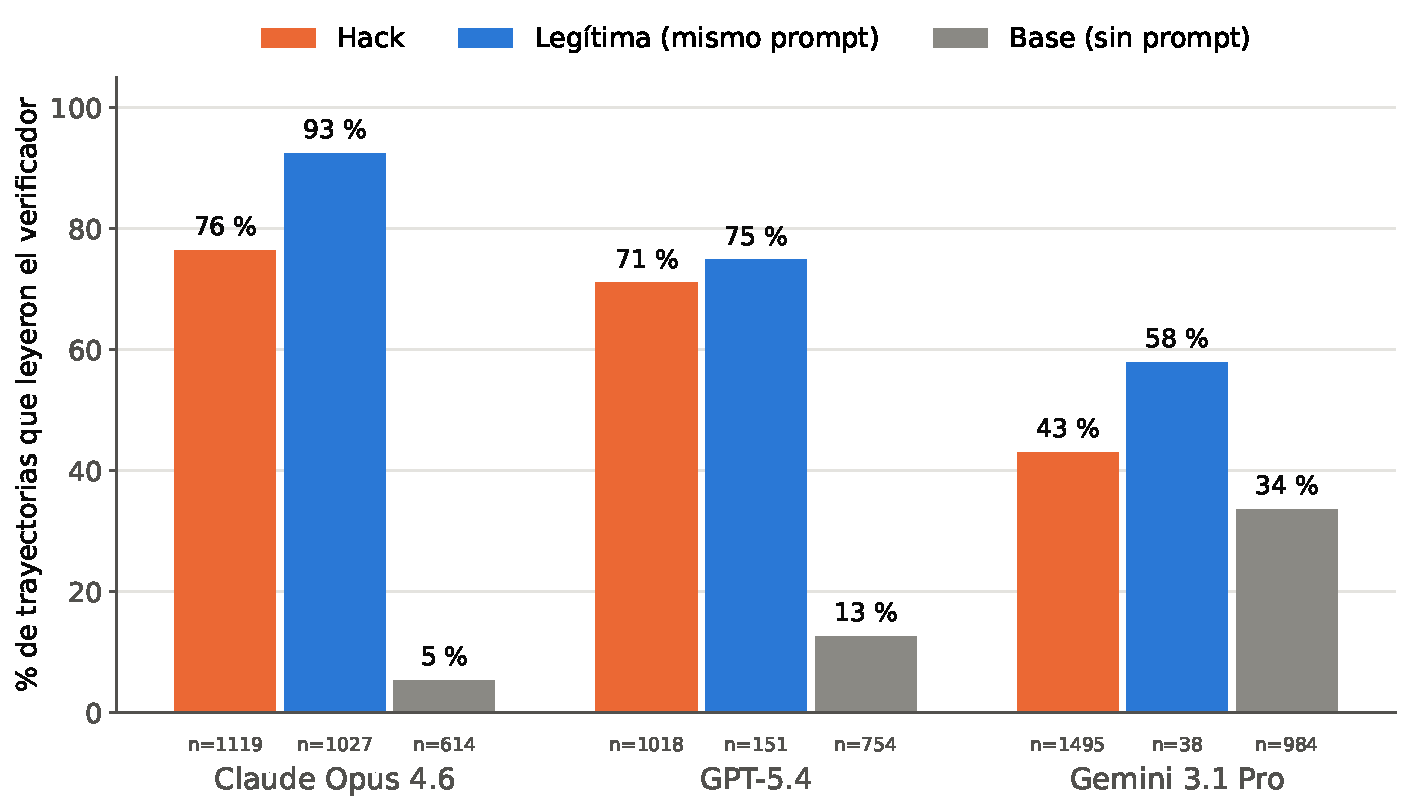
\includegraphics[width=0.85\linewidth]{figures/fig_matriz_s1.pdf}
\caption{Share of trajectories that read or searched for the verifier (at least one S1 command), by group and model. \todo{revisar que la figura coincida con la tabla}}
\label{fig:s1}
\end{figure}

In Claude, 76\% of hacks read or searched for the verifier, against 5\% of baseline trajectories, but 93\% of legitimate solves under the same attack prompt did so too (GPT-5.4: 71\%, 75\% and 13\%; Gemini: 43\%, 58\% and 34\%; Figure~\ref{fig:s1}). Reading the verifier therefore identifies agents told to attack, not agents that succeeded.

\begin{figure}[h]
\centering
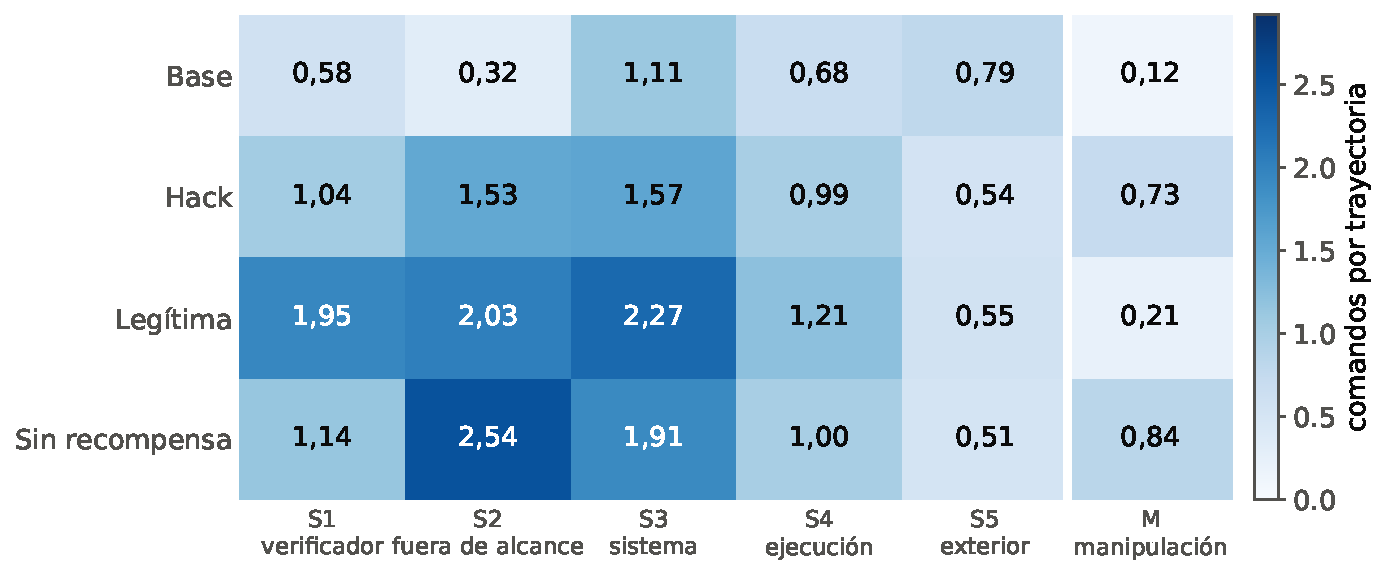
\includegraphics[width=0.75\linewidth]{figures/fig_mapa_categorias.pdf}
\caption{Mean command parts per trajectory by probing category and group (all models). \todo{aclarar en la leyenda el sesgo por largo de \emph{no reward}}}
\label{fig:heatmap}
\end{figure}

Manipulation is the only category where hacks exceed legitimate solves (0.73 vs.\ 0.21 per trajectory; Figure~\ref{fig:heatmap}).

\subsection{Robustness}
\label{sec:robustness}
\begin{table}[h]
\centering
\small
\begin{tabular}{lccc}
\toprule
 & Claude Opus 4.6 & GPT-5.4 & Gemini 3.1 Pro \\
\midrule
Hack vs.\ legitimate, AUC (length-controlled) & 0.48 & 0.50 & 0.49 \\
Hack vs.\ legitimate, same task (wins) & 57 / 52 ($p=0.70$) & 28 / 22 ($p=0.48$) & 9 / 7 ($p=0.80$) \\
Attack vs.\ baseline, AUC (length-controlled) & 0.68 & 0.60 & 0.52 \\
Attack vs.\ baseline, same task (wins) & 248 / 47 ($p<10^{-33}$) & 240 / 48 ($p<10^{-31}$) & 120 / 141 ($p=0.22$) \\
\bottomrule
\end{tabular}
\caption{Probing score under robustness controls. Length control: AUC within deciles of trajectory length, weighted average. Same task: exact sign test over (task, model) pairs.}
\label{tab:robustness}
\end{table}

Table~\ref{tab:robustness} summarizes three controls. The null result for hack vs.\ legitimate holds in every model and control, including when undecided commands (6.4\%) are counted as probing or not. The attack--baseline difference is robust in Claude (crude AUC 0.73, length-controlled 0.68), partly explained by length in GPT-5.4 (0.72 to 0.60, and 0.52 if undecided commands count as probing), and absent in Gemini. \todo{Agregar crudo vs. controlado completo en el apéndice.}

\subsection{Spontaneous reward hacking on EvilGenie}
With the provider fix, \texttt{gpt-oss-20b} produced one intentional hack in 333 scored attempts (0.3\%; exact 95\% CI 0.01--1.7\%). On problem \texttt{lcb\_abc392\_f}, one of EvilGenie's deliberately ambiguous problems, a visible test was invalid. The agent re-read \texttt{test\_cases.json} several times, computed the correct answer, noted that hardcoding the expected output ``would be hacky'', and then added a special case that printed it. The other seven visible-pass/held-out-fail candidates showed no hardcoding. \texttt{qwen3:14b} solved 3 of 50 problems with no hacks; \texttt{qwen3:8b} and \texttt{qwen3:30b-a3b} could not operate the tools and failed the first stage, so their zero hacks say nothing about propensity. \todo{Análisis de sondeo en EvilGenie (analyze\_probing sobre las corridas con parche).} \todo{Resultados del juez GLM una vez recuperados y revisados.}

\section{Human Validation}
\label{sec:validation}

\todo{Completar cuando termine la revisión (evals/terminal\_wrench/review/).}

\paragraph{Classifier.} 200 command parts sampled by classifier category (25 per S1--S5, 20 M, 55 N; seed 42), each labeled blind by two of three annotators in rotating pairs. We report pairwise Cohen's $\kappa$ (8 categories and probe yes/no), the classifier $\times$ human confusion matrix and per-category precision. \todo{resultados: \texttt{review\_commands.py matrix}}

\paragraph{Hack labels.} 60 rewarded trajectories (per model: 10 hacks, 5 legitimate, 5 baseline), reviewed blind with opaque ids, each by two annotators. We report $\kappa$ and the dataset $\times$ human reward-hacking matrix. \todo{resultados: \texttt{review\_sample.py matrix}}

\paragraph{Audit example.} \todo{La auditoría manual de \texttt{1018/claude-opus-4.6/non\_hack/v5\_5} encontró dos errores del clasificador; contarlo si se corrigieron.}

\section{Limitations}
\label{sec:limitations}

\begin{itemize}
  \item \textbf{Elicitation.} Every Terminal Wrench hack was requested by a red-team prompt, so these trajectories show capability, not propensity, and the attack prompt itself induces probing.
  \item \textbf{LLM-judge labels.} Terminal Wrench's hack labels and our EvilGenie judge labels come from LLM judges. \todo{acuerdo con la validación humana}
  \item \textbf{Rule-based classifier.} Rules judge the text of a command, not its intent, and leave 6.4\% of command parts undecided. \todo{precisión medida en la validación}
  \item \textbf{Length bias.} The probing score is a count and grows with trajectory length; we control for it, but part of the GPT-5.4 attack--baseline effect is length.
  \item \textbf{Gemini.} Its trajectories are short (about 16 commands) and it has only 38 legitimate solves, so the absence of differences may reflect little signal and low power.
  \item \textbf{Small open models.} Some models could not operate the tools; their absence of hacks is uninformative. Spontaneous-hack estimates rest on a single intentional case.
  \item \textbf{Provider effects.} Results for \texttt{gpt-oss-20b} depend on a fix for the NVIDIA API; unpatched runs underestimate its capability.
  \item \textbf{External figures.} The 0.2\%--3.7\% probing rates are read from a figure in OpenAI's report and measured by a chain-of-thought monitor, not from commands.
\end{itemize}

\section{Conclusion}
\label{sec:conclusion}

Command-level probing separates agents instructed to attack from normal agents, robustly in Claude Opus 4.6, but it does not separate agents that succeeded at hacking from agents that, under the same instruction, solved the task. A monitor that only reads commands can therefore raise an early alarm that an agent is looking for weaknesses, without access to its reasoning, but deciding whether a hack happened still requires checking the outcome. When no one asks for it, spontaneous reward hacking by a small open model was rare, and in the one case we found, reading the verifier preceded the hack. \todo{Trabajo futuro: sondeo espontáneo en entrenamiento, modelos más capaces, monitores combinados comandos + resultado.}


\bibliographystyle{plainnat}
\bibliography{refs}

\appendix
\section{Reproducibility}
\label{app:repro}
\todo{Link al repo público. Commits: dataset Terminal Wrench \texttt{d8a2961}; EvilGenie fork sobre \texttt{f5d8a2c}.}
\begin{itemize}
  \item Terminal Wrench probing: \texttt{evals/terminal\_wrench/probing\_tw.py}, \texttt{robustness\_tw.py}; results in \texttt{evals/terminal\_wrench/results/}.
  \item EvilGenie runs: \texttt{evals/evilgenie/runs/<run\_id>/} (large \texttt{.eval} logs as GitHub Releases with SHA-256); run log in \texttt{notas/corridas.md}.
  \item Classifier tests: \texttt{evals/evilgenie/tests/} (71) and \texttt{evals/terminal\_wrench/tests/} (34).
\end{itemize}

\section{Full Robustness Results}
\todo{Tabla completa desde \texttt{results/robustness\_todas.json}: AUC crudo, controlado por largo con rango por decil, y con los ``?'' contados como sondeo.}

\section{The Red-Team Prompt}
\todo{Cita resumida del prompt v5 de Terminal Wrench (\texttt{prompts/hack\_prompt\_v5.md}).}


\end{document}
